\documentclass[conference]{IEEEtran}
% \usepackage{silence}
% \WarningFilter[newline]{latex}{Underfull}

\usepackage{booktabs}
\usepackage{float}
\usepackage{multirow}
\usepackage{amsthm}
\usepackage{textcomp}
% \usepackage[english]{babel}

\usepackage{ifpdf}
% Enable correct encoding
\ifpdf{}
    \usepackage[utf8]{inputenc}
\fi{}
\usepackage[T1]{fontenc}

\usepackage[pdftex]{hyperref} % Enable hyperlinks
% \hypersetup{hidelinks}

% Citations Package
\usepackage[
    backend=biber,
    style=ieee
]{biblatex}
\addbibresource{citations.bib}

% "theorem" setup
\newtheorem{definition}{Definition}
\newtheorem{question}{Problem Statement}

\title{Deep Learning’s Potential --- Differentiating Between Images of Concepts
and Tangible Objects}


\author{%
    \IEEEauthorblockN{Pratik Bhusal}
    \IEEEauthorblockA{%
        pratik.bhusal@utdallas.edu\\
        \today
    }\\

    \IEEEauthorblockN{Max Xie}
    \IEEEauthorblockA{%
        max.xie@utdallas.edu\\
        \today
    }
}

\usepackage{graphicx}


% 2. Report Presentation (40%): % {{{


%     1. Is the format correct? IEEE two-column style format, with the font name Times
%     New Roman and size 10.

%     2. Are there obvious grammatical errors or incomplete sentences?

%     3. Are there required sections missing? Each report should include title,
%     abstract, introduction, related work, one or more technical sections, one
%     section about empirical analysis, conclusion, and references.

%     4. Does the report contain plagiarism content?

%     5. Is the proposed AI algorithms and/or models described in sufficient detail?

%     6. What is an overall evaluation of the presentation?

%     7. Is there a clear description about the feature extraction process? Are
%     the features clearly described?

% % }}}

% 3. Technical content (50%): {{{

%     1. Does the implementation code include plagiarism content?

%     2. Is the code uploaded?

%     3. Is there any exploratory data analysis?

%     4. Are the research problem and the main tasks clearly described? The
%     students in one team should focus on separate tasks. If some students
%     focused on the same tasks, the differences of their contributions should be
%     described clearly.

%     5. What is the overall level of efforts for the main tasks. Each report
%     should clearly describe which parts of the code were written by the author.
%     The load of coding can be measured by the the time that is required to
%     implement and debug the code. This time will be estimated by the instructor
%     and TA based on an overall evaluation of the code.  If the load of coding is
%     too low (e.g., 2 hours), the level of efforts will be low (e.g, 0.2). If the
%     load of coding is high (e.g., 50 hours), the level of efforts will be high
%     (e.g., 0.9).

%     6. What is the level of originality and creativity about the proposed work?

%         Examples of high originality and creativity are: (1) The proposed work
%         replicates the results of an existing paper and conducts some new
%         empirical analysis not reported in the paper, such as empirical analysis
%         based on new evaluation metrics (e.g., area under curve, area under
%         precision-recall curve) and new datasets not considered in the paper.
%         (2) The proposed work conducts an empirical comparison between the
%         methods proposed in several different papers. (3) The proposed work
%         develops new algorithms or new neural network architectures and
%         demonstrates the effectiveness and/or efficiency of the proposed
%         techniques, in comparison with some baseline methods in real-world
%         datasets. Algorithms and neural network architectures modified from
%         existing ones are also considered as new. (4) The proposed work presents
%         novel applications of AI models that have not been studied in the
%         current literature. (5) The proposed work develops new algorithms and/or
%         models for Kaggle competitions and demonstrates the effectiveness and/or
%         efficiency of the proposed techniques on the kaggle datasets, in
%         comparison with some baseline methods.

%         Examples of low/medium originality and creativity: (1) The proposed work
%         only replicates the results of an existing paper but does not conduct
%         any new empirical analysis. (2) The proposed work implements classic AI
%         models (e.g., logistic regression, linear regression, bayesian neural
%         networks, support vector machines) for classic problems (e.g.,
%         classification, regression) on some benchmark datasets.

% 7. Is there a detailed discussion about how the hyper parameters were turned?
% Have the finalized hyperparameters of all the AI models been reported?

% 8. Are the empirical results discussed in sufficient detail?

% % }}}

\begin{document}
\maketitle



\begin{abstract} % {{{

% TODO: Write this section last. A reasonable way to write an abstract is to
% write a 1 sentence highlight of each of the sections in the paper, then go
% back and smooth it out so it flows cleanly and makes the key points you want.
% <2020-04-09, Pratik Bhusal>

Hello World
\end{abstract} % }}}



\section{Introduction} % {{{

Over the last decade, the field of computer vision has seen massive, almost
routine innovations. Mainstream adoption of applying the theory behind various
image-based tasks have become commonplace. Some examples include, but are not
limited to:

\begin{itemize}
    \item Image Classification: Computer Vision task where one predicts the
        msot likely class given from a set of known labels.
    \item Bounding Box Classification: Given a particular image with a main
        focusing point or even multiple objects, a box bounding the notable,
        known objects are formed based on a set of known classification labels.
    \item Pixel Classification: Given an image each pixel in the figure is
        masked with a particular classification label from a set of known
        possible classes.
    \item Object segmentation: A natural merging of the research, methodology,
        and architecture between bounding box classifications and pixel
        classification. In this computer vision task, for a given image, a
        pixel-for-pixel mask accounts for object that would not only be labled
        in the same class but are still distinct enough entities and be colored
        with different color masks
\end{itemize}

Most impressingly, such convoluted, computationally demanding tasks to achieve
respectable results ahve also seen a recent surge in innovation. Models designed
to work in embedded systems and portable hardware and devices such as standard
smartphones are slowing starting to become commonplace. These arithmetically
efficient nueral network designs have made comparable results to neural network
designs that can easily have over 1000 hidden layers and order of magnitudes
more multiply-and-accumulation units (MACs) and trainable parameters.


However, one caveat to all this forward momentum in classification tasks over
the last decade and even possibly the last few years in an almost universal,
almost monopolistic focus on tangible objects.


Rather than following the norm, a call to question an alternative outlook forms.
Instead of focusing on what can be percieved by sight or touch, concepts are an
anomoly to human anomoly to the human senses.

For example, consider the situation where there is a singular orange 2 meters
afar. While it is easily descernable that the object in the distance is that of
an orange, the notion of what the number ``1'' is still is both alluding and
alluring. Even though there is no true tangible representation of ``1'' itself
without the aid of a tangible middleman, biological beings are still able to
descern the underlying information. This innate ability to simply ``know'' is
what this paper will attempt uncovering for the remainder of the report.


% }}}



\section{Motivation} % {{{

To clarify some necessary verbage used and will be used for the rest of the
paper, a ``tangible [object]'' will be defined as the following:

\begin{definition}[Tangible Object]

    An object that is capable of being perceived especially by the sense of
    touch.

\end{definition}

Likewise, this paper will define a ``concept'' with the following definition:


\begin{definition}[Concept]

    An abstract or generic idea generalized from particular instance or
    instances.%
    \label{ConceptDefinition}
\end{definition}

The motivation for this alternative approach to computer vision has 2 parts or
folds for interest.


\subsection{Fold 1: Novelty}

As mentioned before, most if not all nueral network designs utilized for
classification tasks have been focused on tackling some means of labeling
for tangible objects. By even slightly twisting the challange, a new region of
computer vision classification tasks is finally untapped.

This bewilderment of the underlying premise leads us to the initual formulation
of our problem statement:


\begin{question}
    Is it feasible for an artificial agent to be trained to  distinguish between
    a concept and a tangible object?
\end{question}


\subsection{Fold 2: Result Maxmimation With Minimal Resources}

In computer vision classification tasks, computationally efficient networks
exist to perform the same or similar level as their more demanding counterparts.
Naturally, interest arise on its own merits on ho well a ``simple'' model can
``understand'' the nuance  and potentially layed abstraction that a concept can
be generalized from. This approach can also hint at a fundamental notion of
concepts not necessarily being as demanding a task to fully grasp even with
how deterministic neural networks perform. Hence, while it may be questionable
how more refined the formulation, a more interesting question to ask and what
this paper will focus on answering is the following problem statement:


\begin{question}
    Is it feasible to train a artificial agent designed around to have  minimize
    computational resources (MACs) while still making a model accuratly and
    precisely distinguish between a concept and a tangible object?%
    \label{question:MainQuestion}
\end{question}

The coming sections will focus on answering problem
statement~\ref{question:MainQuestion}. The paper will analze established network
architectures as a baseline reference implementation, discuss the methodologies
used to answer the above question from inception to implementation, analyze the
results of the implemented models designed to work with the chosen dataset, and
finally make concluding statements based on the provided findings.

% }}}



\section{Related Works} % {{{


\subsection{ResNet V2 (ResNet-50)}


\subsection{MobileNet V2}


\subsection{MobileNet V3}


% }}}



\section{Proposed Approach} % {{{


\subsection{Dataset}\label{ProposedApproach-Dataset}


\subsection{Pre-Processing}

\subsubsection{Stratified Sampling}


\subsubsection{Classification Relabling}


\subsubsection{Image Cropping}


\subsubsection{Image Normalization}

\subsection{Modifying ResNet V2}


\subsection{Modifying MobileNet V2}


\subsection{Modifying MobileNet V3}

% }}}



\section{Results} % {{{


\subsection{ResNet V2}


\subsection{MobileNet V2}


\subsection{MobileNet V3}


\subsection{Network Comparison}


% }}}


\section{Shortcomings} % {{{


\subsection{Dataset}\label{Shortcomings-Dataset}


As mentioned in Section~\ref{ProposedApproach-Dataset}, the main reason for
choosing MNIST and Fashion MNIST as the datasets to answer problem
statement~\ref{question:MainQuestion} was due to their similarities. Their
naturally equivalent structure from Fashion MNIST's purpose to act as a
drag-and-drop replacement for MNIST in image classification tasks make it an
easy choice to pair with for this research investigation. However, there are
drawbacks to using this particular dataset style or even what information is
even in the chosen datasets.


\subsubsection{Greyscale Dataset by Default}

Instead of MNIST and Fashion MNIST being colored image datasets that have been
preprocessed into greyscale images to reduce the number of mathmatical
operations to determine a classification, the images were already in greyscale.
The immediate benefits is less less overall processing, but this dataset
approach also comes with its own fair share of disadvantages.



\begin{figure}[H]
  \centering
  
\includegraphics[width=0.8\linewidth]{figures/placeholder.png}
  \caption{Greyscaled ImageNet figure~\cite{imagenet2012}}%
  \label{fig:GreysclaeImageNetExample}
\end{figure}

One main cause for concern is that the MNIST or MNIST-like datasets do not have
much if any noise in the images from what would have been created when doing a
grayscaling convertion from a colored image.

Image~\ref{fig:GreysclaeImageNetExample} exemplifies this particular issue where
noticable splotches are clearly visible. Even when performing a normalization
step after greyscaling, there was still discernable, residual noise from the
greyscaling operation. These ``splotches'' could easily identify that a
particular image belonged to one label/superlabel or the other label/superlabel.
Hence, a decision was made to forego such images was made in the hopes to
minimize the always looming concern of pixel memorization over image
recognition.




\subsection{Preprocessing}

A common step in computer visision image classification tasks is to rotate a
given image by 90\textdegree{} clockwise or counter-clockwise, horizontally
flipping the image or vertically flip the image.


\begin{figure}[H]
  \centering
  
\includegraphics[width=0.8\linewidth]{figures/placeholder.png}
  \caption{Original Fashion MNIST Image~\cite{fashion_mnist}}%
  \label{fig:FashionMNIST-OriginalImage}
\end{figure}


\begin{figure}[H]
  \centering
  
\includegraphics[width=0.8\linewidth]{figures/placeholder.png}
  \caption{Flipped Fashion MNIST Image~\cite{fashion_mnist}}%
  \label{fig:FashionMNIST-RotatedImage}
\end{figure}

For example, consider Image~\ref{fig:FashionMNIST-OriginalImage} and its rotated
counterpart Image~\ref{fig:FashionMNIST-RotatedImage}. While it may seem
intuitive to a biological being that both images represent the same object, an
artifical nueral network may not. The artificial agent does not initially view a
given image in the same perspective as a human being. Initially, all it is aware
of is the pixel values for each channel the image has. In due time, the agent
may reach a critical point where it is at least of acceptable accuracy as a
human if not already classiffy images well enough that it is faster than a
biological agent. However, a problem arises where the image used to represent a
concept is orientation sensitive.


\begin{figure}[H]
  \centering
  
\includegraphics[width=0.8\linewidth]{figures/placeholder.png}
  \caption{Original MNIST Image~\cite{mnist_dataset}}%
  \label{fig:MNIST-OriginalImage}
\end{figure}


\begin{figure}[H]
  \centering
  
\includegraphics[width=0.8\linewidth]{figures/placeholder.png}
  \caption{Flipped MNIST Image~\cite{mnist_dataset}}%
  \label{fig:MNIST-RotatedImage}
\end{figure}

Consider the following example rotation above.
Figure~\ref{fig:MNIST-OriginalImage} is easily discernable as the number ``1''.
However, a correct classification for Figure~\ref{fig:MNIST-RotatedImage} is
less so. ONe may easily mistake it as a dashed line (``---'') rather thn a
transposed number ``1''. WHile it may have a vertical symmetry, the only other
number in the dataset with this property is ``3.''

In fact, performing rotating an image of the number ``6'' may confuse
both the artifical agent and the biological agent. Ultimately, it will case them
to predict the transposed figure  depicts the number ``9''. Hence,

Hence, a decision was made to forego this type of image preprocessing  to
minimize the confusion  even if it meant there was a cost to generation a more
exhausive tangible object dataset.

% }}}


\section{Future Endeavors} % {{{


\subsection{Colored Datasets} % {{{

As mentioned before, one of the report's biggest setbacks was the lack of
avalibility in a colored datast that can be used to represent an image of some
concept. During the concoluding era of the paper's investigation for Problem
Statement~\ref{question:MainQuestion}, the street view house numbers (SVHN)
dataset came up in discussion~\cite{stree_view_house_numbers_dataset}. As there
are 2 possible format for this dataset, the following sections will only cover
the 32$\times$32 RGB singular format of the dataset.


\begin{figure}[H]
  \centering
  
\includegraphics[width=0.8\linewidth]{figures/placeholder.png}
  \caption{Sample Image from SVHN Dataset~\cite{stree_view_house_numbers_dataset}}%
  \label{fig:SVHN-SingularNumber}
\end{figure}

As shown in Figure~\ref{fig:SVHN-SingularNumber}, this is \textit{almost}
equivalent to the traditional MNIST dataset. The larger 32$\times$32 instead of
MNIST's standard 28$\times$28 image dimensions and the 3 color channels instead
of only a greyscale image channel are the main drawing points to utilizing this
dataset.

As stated in Section~\ref{Shortcomings-Dataset}, the investigation avoided
mixing colored datasets and the already aggregated MNIST or MNIST-like datasets
in avoiding the possibly of the greyscaling process would leave artifacts that
could not exist in an already greyscaled dataset. By utilizing this dataset, it
is not feasible to utilize a colored dataset to represent a superlabel for
concepts and to utilize a dataset such as CIFAR-10 or CIFAR-100 (32$\times$32 colored
images datasets) with a superclassification of tangible object images.
Critically, the street view house numbers dataset allows further investigation
about the importance of color having an impact on the decision-making process
that distinguishes between a concept and a tangible object.


\begin{figure}[H]
  \centering
  
\includegraphics[width=0.8\linewidth]{figures/placeholder.png}
  \caption{Sample Image from SVHN Dataset with distracting digits~\cite{stree_view_house_numbers_dataset}}%
  \label{fig:SVHN-ImageWithDistractingDigits}
\end{figure}


As with any dataset, there is always a caveat. In
Figure~\ref{fig:SVHN-ImageWithDistractingDigits}, partial portions of the
different number are visible within the given image. There is a possibility that
the model may try to learn around the distracting numbers and cause an incorrect
classification. Some amount of cropping will be required, but the dataset
overall helps over the doors for more colorful representation of concepts.

% }}}

\subsection{Alternative Network Architectures}% {{{

Computationally demanding yet more representative models could provide loss
values that outperform the 3 resoure-lite designs this report tested the
training methodoloy upon. Section~\ref{NasNet} and Section~\ref{Inception-V2}
will go over 2 notable designs that compliment the desire to provide a somewhat
computationally efficient model or further avoid issues of an image not taking
the entire pixel space to represent the main piece.


\subsubsection{Neural Architecture Search Network (NASNet)}\label{NasNet}


\begin{figure}[H]
  \centering
  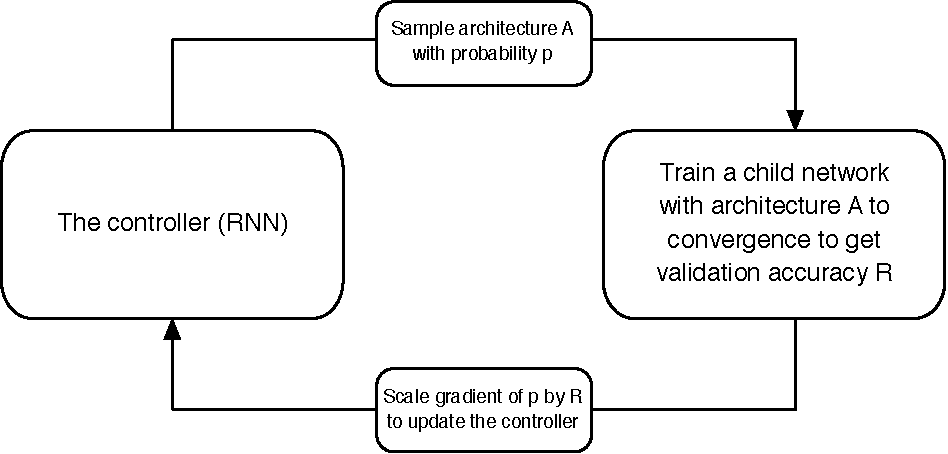
\includegraphics[width=\linewidth]{figures/NAS-Diagram.pdf}
  \caption{NASNet Model Formulation Process~\cite{nasnet_paper}}%
  \label{fig:NasNet-Procss}
\end{figure}



With another artifial nueral architecture design, the particular model provides
a unique means of transfer learning. As depicted in
Fiture~\ref{fig:NasNet-Procss}, rather than transfering over parameters to
aid with a similar classification task, the arhitectural building block is
instead passed over to the more computationally advanced
model. The model recieves an initially smaller dataset in
terms of image input dimension size. When it comes to colored image
classification tasks, after training the network on the CIFAR-10 dataset, it has
shown a remarkable 74\% accuracy when intentionally designed for mobile
devices~\cite{nasnet_paper}.  With how extensible the architecture is, more
computationally advanced approaches can make strides in differentiating the
difference between concepts and tangible objects.


\subsubsection{Inception V2}\label{Inception-V2}



One of the major faults in the MNIST dataset is the variance in shape and how
much of the image is taken up by the object. Thankfully, the Inception family of
networks are designed around the issue that a fixed kernel size cannot
accurately represent all possible ways the parent space of the main object takes
up relative to the amount of background or unnecesary additional information.


% \begin{figure}[H]
%   \centering
%   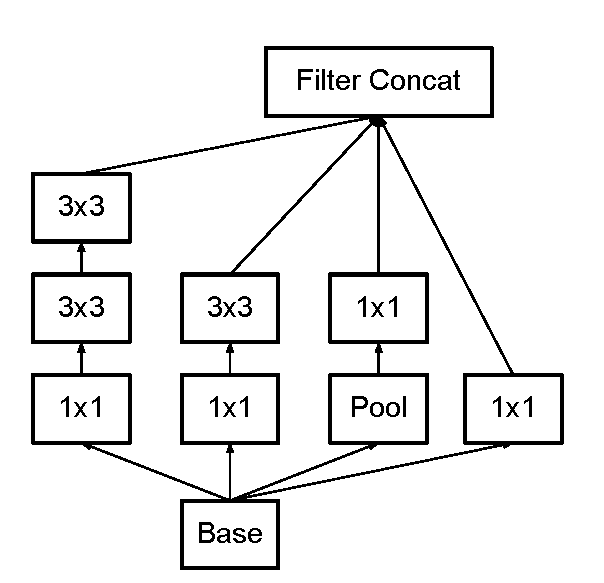
\includegraphics[width=0.8\linewidth]{figures/inceptionv2_block.pdf}
%   \caption{Inception V1 Module~\cite{inception_v1_paper}}
% \end{figure}

Inceptioon V1 layed the groundwork is by utilzing multiple mini-networks to
replace the fixed 3$\times$3. Once  processed, the mini-networks are filtered
and concatenated together~\cite{inception_v1_paper}.


\begin{figure}[H]
  \centering
  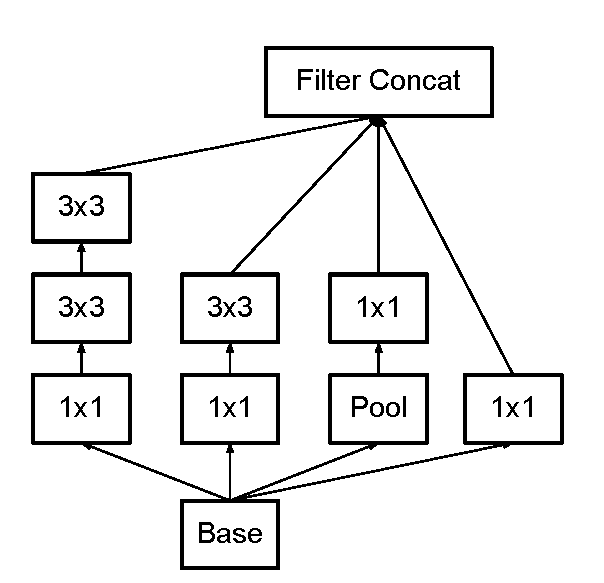
\includegraphics[width=0.8\linewidth]{figures/inceptionv2_block.pdf}
  \caption{Inception V2 Module~\cite{inception_v2_paper}}%
  % \label{fig:InceptionV2-Block}
\end{figure}


Inception V2 takes the original design of the Inception V1 and tries to minimze
the input dimension alterations. A new set of 2 3$\times$3 convolution
mini-network now exists where the orignal single 5$\times$5 convolution
mini-network existed~\cite{inception_v2_paper}. The network's main argument is that input dimension
alternations where large convolutions cause a given input to go through a
``representational bottleneck'' makes for an overall weaker artifical agent. By
taking this miniaml alterations approach where the max convolution size is now
3$\times$3, Inception V2 avoids the issue that many other models go headfirst
into.



% }}}

\subsection{Concept Denotation and Connotation}% {{{


Arguably the biggest point of criticism arises from how the report \textit{only}
focused on utilizing arabic numerals --- a specific example from the domain of
possible ways to represent a concept. One aspect of research that was not
covered in this report but may be able to in the future is the dichotomy betwen
what the image of the concept corresponds to and the underlying connotations
that the image exeplifies.


\begin{figure}[H]
  \centering
  
\includegraphics[width=0.8\linewidth]{figures/placeholder.png}
  \caption{Image of the fruit Apple}%
  \label{fig:AppleFruit}
\end{figure}


\begin{figure}[H]
  \centering
  
\includegraphics[width=0.8\linewidth]{figures/placeholder.png}
  \caption{Image of the the Apple Company Logo}%
  \label{fig:AppleCompanyLogo}
\end{figure}

Consider the following thought experiemtn. Image~\ref{fig:AppleFruit} is an
image of the fruit apple. Image~\ref{fig:AppleCompanyLogo}. While both may have
the same name, their representations are far as can be. MOre importantly, even
though the Apple company logo represents an abstraction of a particular
instance (and hence fits within the domain defined by
Definition~\ref{ConceptDefinition}), it has an underlying significance that any
authentic product embellished with the logo has a high level of quality in terms
of design and perforce that is backed by a trillion dollar company. While the
paper did not explore this concept region in the overall domain, for a computer
vision task this will help further advance the similarities and difference
between concepts and tangible objects in terms of signaling the the underlying
meaning behind what is visible.


% }}}


% }}}



\section{Conclusion} % {{{

% TODO: Write 1 – 2 sentences on each of motivation, design, training and
% implementation. Do this after putting together the other sections but before
% the abstract. <2020-04-09, Pratik Bhusal>


We did things.


% }}}



{\hbadness=10000\printbibliography}

\appendix

\end{document}
